\documentclass[pdftex,12pt,a4paper]{article}
\usepackage[pdftex]{graphicx}
\usepackage{xcolor}
\usepackage{marginnote}
\usepackage{enumitem}
\usepackage[bottom=1.5cm, outer=5cm, inner=2cm, heightrounded,
marginparwidth=4cm, marginparsep=0.5cm]{geometry}

\begin{document}
    % Custom title page
    \begin{titlepage}
        \begin{center}
            
\includegraphics[width=5cm]{figures/kulogo}\\[1cm]
            {\Large \bfseries
                Spring 2014\\
                Computer Networks\\
                CMPE323\\[1cm]
            }
            {\large \bfseries
                \noindent Laboratory Experiment No. 4: Introduction to Internet
                Protocol (IP) and Class-less Inter-domain Routing (CIDR)\\[1cm]
            }
        \end{center}

        \noindent \textbf{Aims and Objectives:}
            \begin{itemize}[leftmargin=4cm]
                \item Introduce students to a scalable best-effort end-to-end
                    routing architecture.
                \item Introduce students to IP versions 4 and 6 as examples of
                    such routing architecture.
                \item Allow students to manually craft their first IPv4 and
                    IPv6 packets (according to IETF standards RFC791 and RFC2460
                    respectively).
                \item Practically verify the correct routing
                    behavior according to the CIDR architecture (IETF standard
                    RFC4632).
            \end{itemize}
            \vspace{0.5cm}

        \noindent \textbf{Materials Required:}
            \begin{itemize}[leftmargin=4cm]
                \item IP routers,
                \item Ethernet switches,
                \item PCs with Ethernet adapters,
                \item and straight-through/crossover/rollover cables.
            \end{itemize}
            \vspace{0.5cm}

        \noindent \textbf{Change Log:}
            \begin{itemize}[leftmargin=4cm]
                \item 11-3-2014: original document -- mkhonji.
            \end{itemize}
    \end{titlepage}
    \newpage

    % Lab script content
    \section{Introduction}
        Before we discuss why Internet Protocol (IP) is useful, we will first:
        \begin{itemize}
            \item recap what we have learned so far with regards to Ethernet
                broadcast domains and why the scalability problem that
                introduce,
            \item then introduce how IP and CIDR solve the scalability issues of
                broadcast domains.
            \item Additionally, we will briefly touch the main differences
                between the two most popular version of IP, namely versions 4
                and 6 respectively.
        \end{itemize}

        \subsection{Why is Ethernet not enough?}
            In previous labs 2 and 3, we learned that:
            \begin{itemize}
                \item In order for Ethernet to function, it \emph{sometimes}
                    has to broadcast messages to all connected devices. This
                    introduced the notion of a \emph{broadcast domain}.
                \item If we connect too many nodes or PCs to a set of
                    inter-connected Ethernet switches, we will create a huge
                    broadcast domain.
                \item Huge broadcast domains are a bad idea as they introduce
                    efficiency problems (e.g. loss of bandwidth), as well as
                    the linear growth of the MAC address table as number of
                    communicating nodes increase. Additionally, security issues
                    (e.g. some attacks thrive in broadcast domains).
                \item To reduce the size of broadcast domains, we should
                    segregate them into smaller broadcast domains by:
                    \begin{itemize}
                        \item Connecting nodes/PCs to isolated physical
                            Ethernet switches. This way a PC can only talk to
                            other PCs that are connected to the \emph{same}
                            switch (but cannot talk to other PCs that are
                            connected to \emph{different} switches).
                        \item Or by simply using Virtual LANs (VLANs) to
                            decouple the broadcast domain segregation from the
                            underlying physical network layout. This way, we
                            can set up any broadcast domain boundaries by
                            simply configuring the Ethernet switches (e.g. no
                            need to physically disconnect/connect cables;
                            thanks to IEEE 802.1Q tags).
                    \end{itemize}
                \end{itemize}

                However, the PCs in the different broadcast domains remained
                isolated and had no means of communication between each other.
                If we stop here, then large networks such as the Internet will
                not be possible. In order to allow large networks to exist, we
                need to find a method to inter-connect isolated broadcast
                domains while also maintaining broadcast domain boundaries.

                The question is: can we allow PCs from different broadcast
                domains to communicate with each other in a scalable manner
                (i.e. while maintaining small-sized broadcast domains)? The
                answer to the question is ``yes'' and the mechanism is
                introduced in the subsequent sections of this lab.

        \subsection{What are IP and CIDR? How do they address the
        scalability problems?}
            The primary objective of the IP protocol is to facilitate an
            addressing scheme that is aggregatable in order to allow
            hierarchal routing.

            Simply put, Class-less Inter-domain Routing (CIDR) is basically a set of rules
            that govern how should equipments behave based on information that
            is provided in the IP packets.

            Figure \ref{fig:cidr} depicts an IP example with focus on the
            routing table. Notice how the number of IP addresses in the IP
            routing table is independent of the number of communicating
            PC.

            Additionally, routers (i.e. R$1\ldots5$) do not forward broadcasts.
            For example, if the PC with the IP address \texttt{10.0.0.1} wishes
            to send a packet to \texttt{10.1.0.3}, it only needs to forward the
            packet to R3's \texttt{eth1} interface by encapsulating it in a MAC frame
            with a destination MAC address equivalent to the MAC address of
            R3's \texttt{eth1} interface.

            \begin{figure}[tbh]
                \centering
                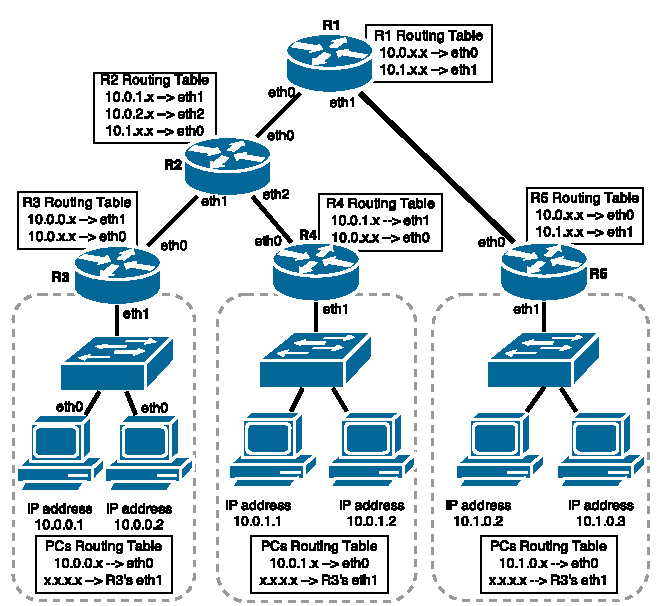
\includegraphics[width=0.9\textwidth]{figures/cidr}
                \caption{An IPv4 network with focus on the IPv4 routing table.
                \textbf{Note:} the figure shows interface IDs in the
                routing table, which is not always the case; in Ethernet
                networks (or any broadcast network), the next-hop is the IP address
                of the next-hop interface. However, interface IDs are shown for
                space efficiency.}
                \label{fig:cidr}
            \end{figure}

            \textbf{Notes:} 
            \begin{itemize}
                \item This lab will focus on IP packets over Ethernet, but it
                    doesn't have to be this way. IP packet can be carried over
                    a variety of layer 2 protocols such as FrameRelay, HDLC,
                    TokenRing, etc.
                \item In theory, and in order for IP routing to function,
                    intermediate devices that facilitate such routing (i.e. IP
                    routers) don't need to have IP addresses for their own
                    interfaces (e.g. R3's \texttt{eth1} interface doesn't need
                    to have an IP address). All routers need is a routing
                    table, connectivity with next hops at layer 2, and the
                    ability to process IP packets accordingly (e.g.
                    decrementing IP header's TTL, updating IP header's
                    checksum, etc). The routing table needs to basically map
                    destination IP-network addresses against a layer-2
                    next-hope layer 2 address (as in case of broadcast domains)
                    or router's exit point interface (in case of point-to-point
                    networks). 
                \item However, configuring MAC addresses as next-hope addresses
                    will make the IP routing table configuration dependent on
                    the underlying layer 2 protocol. It is therefore desirable
                    to follow a simpler approach were layer 2 protocol details
                    are abstracted. This is also a problem if associated
                    Ethernet network adapters are updated as their MAC
                    addresses will change and therefore all routing entries
                    need to be updated accordingly (which adds administrative
                    overhead).
                \item Such layer 2 abstraction is achieved as follows:
                    \begin{itemize}
                        \item Instead of populating routing tables with entries
                            that map IP-network addresses against next-hop MAC
                            addresses, next-hop IP addresses are used instead
                            of next-hop MAC addresses.
                        \item In order to resolve the next-hop IP addresses
                            into next-hop MAC addresses, the ARP protocol is
                            used automatically by routers and nodes alike.
                    \end{itemize}
            \end{itemize}


        \subsection{Different versions of IP}
            There are two version of IP in today's production networks, namely
            IPv4 and IPv6.

            \subsubsection{IPv4}
                The primary service that the IPv4 provides is an aggregatable
                source and destination IP addresses, which is a 32bit number.
                However, the IPv4 header provides additional options that are
                beyond the scope of this lab, which are (see Figure
                \ref{fig:ipv4}):
                \begin{itemize}
                    \item 4 bits version --- \texttt{0100} in binary to
                        indicate that the subsequent bits to be interpreted as
                        IPv4.
                    \item 4 bits header length --- the unit is in 32bits, and
                        the minimal header length is $5 \times 32$ bits. For
                        example, for the smallest header (i.e. one without
                        optional fields), the value is \texttt{0101} in binary.
                    \item 8 bits for type of service --- this is used for
                        Quality of Service (QoS) related topics which is beyond
                        the scope of this lab. For the purpose of this lab, we
                        will assume a value of 0 for this field.
                    \item 16 bits total length --- total number of octets for
                        the IPv4 header as well as its payload.
                    \item 16 bits packet identification --- this is used for
                        fragmentation purposes which is beyond the scope of
                        this lab. For the purpose of this lab, we will assume a
                        value of 0.
                    \item 3 bits flags --- this is used for fragmentation
                        purposes which is beyond the scope of this lab. For the
                        purpose of this lab, we will assume a value of 0.
                    \item 13 bits fragment offsets --- this is used for
                        fragmentation purposes which is beyond the scope of
                        this lab. For the purpose of this lab, we will assume a
                        value of 0.
                    \item 8 bits time to live --- this is a number that
                        indicates maximum number of routes this packet can
                        cross before its death, which helps in avoiding
                        eternally looping packets. Each router in the path
                        decrements this value by 1, and once it reaches 0 the
                        packet will be discarded.
                    \item 8 bits next protocol --- this is a number that
                        identifies the protocol ID of the data in the payload
                        of this IP packet.
                    \item 16 bits header checksum --- this allows routers and
                        hosts to detect errors in packets and discard them if
                        errors exist. The header checksum algorithm is simple
                        and is as follows:
                        \begin{quote}
                            ``The checksum field is the 16 bit one's complement of the
                            one's complement sum of all 16 bit words in the header.
                            For purposes of computing the checksum, the value of the
                            checksum field is zero.'' --- Source RFC791.
                        \end{quote}

                        For the purpose of verifying the checksum, the 16 bit
                        one's complement sum of all 16 bit words is computed,
                        including the header's checksum. If the answer is 0,
                        the header is deemed valid.

                    \item 32bit source IP address.
                    \item 32bit destination IP address.
                    \item Variable length options --- this beyond the scope of
                        this lab, and we will not include them in our headers.
                \end{itemize}

                \begin{figure}[tbh]
                    \centering
                    \begin{verbatim} 0                   1                   2                   3
 0 1 2 3 4 5 6 7 8 9 0 1 2 3 4 5 6 7 8 9 0 1 2 3 4 5 6 7 8 9 0 1
+-+-+-+-+-+-+-+-+-+-+-+-+-+-+-+-+-+-+-+-+-+-+-+-+-+-+-+-+-+-+-+-+
|Version|  IHL  |Type of Service|          Total Length         |
+-+-+-+-+-+-+-+-+-+-+-+-+-+-+-+-+-+-+-+-+-+-+-+-+-+-+-+-+-+-+-+-+
|         Identification        |Flags|      Fragment Offset    |
+-+-+-+-+-+-+-+-+-+-+-+-+-+-+-+-+-+-+-+-+-+-+-+-+-+-+-+-+-+-+-+-+
|  Time to Live |    Protocol   |         Header Checksum       |
+-+-+-+-+-+-+-+-+-+-+-+-+-+-+-+-+-+-+-+-+-+-+-+-+-+-+-+-+-+-+-+-+
|                       Source Address                          |
+-+-+-+-+-+-+-+-+-+-+-+-+-+-+-+-+-+-+-+-+-+-+-+-+-+-+-+-+-+-+-+-+
|                    Destination Address                        |
+-+-+-+-+-+-+-+-+-+-+-+-+-+-+-+-+-+-+-+-+-+-+-+-+-+-+-+-+-+-+-+-+
|                    Options                    |    Padding    |
+-+-+-+-+-+-+-+-+-+-+-+-+-+-+-+-+-+-+-+-+-+-+-+-+-+-+-+-+-+-+-+-+\end{verbatim}
                    \caption{Internet Protocol (IP) version 4 header format --- Source RFC791.}
                    \label{fig:ipv4}
                \end{figure}

            \subsubsection{IPv6}
                One of the main problems with IPv4 is that its address space
                was too small as its designers did not expect IPv4 to gain such
                massive popularity. In the early 1990s, it was known that
                IPv4's 32bit address space is not enough.

                IPv6 solves this problem by using 128 bit address space which
                provides a extremely larger address space. 

                Additionally, IPv6 is a much simpler protocol than IPv4 and
                fixes a number other issues with the IPv4 which is as follows
                (see Figure \ref{fig:ipv6}):
                \begin{itemize}
                    \item Header length field is removed. As far as routers are concerned, the IPv6 header is
                        fixed length. Optional fields are provided as
                        extensions (beyond the scope).
                    \item Removes the checksum field as it slows down routing
                        (as routers would need to recompute the checksum
                        every time they decrement the TTL in IPv4). The
                        checksum is also redundant as they exist in layer 4
                        headers (e.g. TCP and UDP).
                    \item Time to live is renamed into \emph{hop limit} which
                        is a more accurate terminology.
                \end{itemize}

                Because IPv6 addresses are long, they are represented in hex in
                groups of 16 bits. For example, the following is an example of
                an IPv6 address:
                \texttt{FD00:0000:0000:0000:0000:0000:0000:0001}. Additionally,
                and since sequences of 0s are common in IPv6 addresses, a
                sequence of consecutive 0s can be abbreviated by \texttt{::} as
                follows: \texttt{FD00::1}.

                \begin{figure}[tbh]
                    \centering
                    \begin{verbatim} 0                   1                   2                   3
 0 1 2 3 4 5 6 7 8 9 0 1 2 3 4 5 6 7 8 9 0 1 2 3 4 5 6 7 8 9 0 1
+-+-+-+-+-+-+-+-+-+-+-+-+-+-+-+-+-+-+-+-+-+-+-+-+-+-+-+-+-+-+-+-+
|Version| Traffic Class |           Flow Label                  |
+-+-+-+-+-+-+-+-+-+-+-+-+-+-+-+-+-+-+-+-+-+-+-+-+-+-+-+-+-+-+-+-+
|         Payload Length        |  Next Header  |   Hop Limit   |
+-+-+-+-+-+-+-+-+-+-+-+-+-+-+-+-+-+-+-+-+-+-+-+-+-+-+-+-+-+-+-+-+
|                                                               |
+                                                               +
|                                                               |
+                         Source Address                        +
|                                                               |
+                                                               +
|                                                               |
+-+-+-+-+-+-+-+-+-+-+-+-+-+-+-+-+-+-+-+-+-+-+-+-+-+-+-+-+-+-+-+-+
|                                                               |
+                                                               +
|                                                               |
+                      Destination Address                      +
|                                                               |
+                                                               +
|                                                               |
+-+-+-+-+-+-+-+-+-+-+-+-+-+-+-+-+-+-+-+-+-+-+-+-+-+-+-+-+-+-+-+-+\end{verbatim}
                    \caption{Internet Protocol (IP) version 6 header format --- Source
                    RFC2460.}
                    \label{fig:ipv6}
                \end{figure}

        \subsection{CIDR}
            In order to aggregate groups of IP addresses, subnet masks are
            used. Quite simply, a subnet mask is either:
            \begin{itemize}
                \item 32 bit number in IPv4,
                \item or 128 bit number in IPv6.
            \end{itemize}

            The subnet mask is a sequence of bits that help routers understand
            which portions of a given IP address to be used for the routing
            lookup (network part), and which parts to be ignored (host part).

            For example, the following IPv4 addresses are represented in binary
            as follows:
            \begin{itemize}
                \item 10.0.0.1 is represented in binary as:
                    \texttt{00001010.00000000.00000000.00000001}.
                \item 10.0.0.2 is represented in binary as:
                    \texttt{00001010.00000000.00000000.00000010}.
                \item 10.0.254 is represented in binary as:
                    \texttt{00001010.00000000.00000000.11111110}.
            \end{itemize}

            And if we wish to configure the router to aggregate all of the
            above addresses into a single routing table entry, we will need the
            following routing entry:
            \begin{itemize}
                \item Network IPv4 address:
                    \texttt{00001010.00000000.00000000.00000000}.
                \item Subnet mask: \texttt{11111111.11111111.11111111.00000000}
                \item Exit interface or next hop address.
                \item Metric (the lower the more preferred the routing table entry).
            \end{itemize}

            The IPv4 router then, generally, performs the routing task upon the reception
            of every IPv4 packet:
            \begin{itemize}
                \item Extract the IPv4 destination address from the packet.
                \item Perform a bit-wise \texttt{AND} operation against longest
                    subnet mask. This will result in returning the network IP
                    address (where host bits are 0s).
                \item Compare the resultant network IP address against the
                    network IP address of the routing entry that is associated
                    to the applied subnet mask.
                \item If the resultant network IP address matches the routing
                    table entry's network IP address, then execute it by
                    forwarding the received packet towards the exit interface
                    or the next-hop address.
                \item In case multiple routing entries are matched, execute the
                    one with the lowest metric.
                \item In case there are multiple routing table entries with the
                    \emph{same} metric, then routers sometimes load balance
                    across them (i.e. sometimes execute one, while some other
                    times execute the other one). This is called equal-cost
                    load balancing. Unequal-cost load balancing exists but it's
                    beyond the lab's scope.
            \end{itemize}

            Historically (early 1980s), IPv4 addresses were aggregated using
            subnet masks that were derived from the leading bits of the subject
            IPv4 address. For example, IPv4 addresses that begin with the
            binary sequence \texttt{0} were considered to have a subnet mask of
            255.0.0.0 (also known as class \emph{A} addresses), and IPv4
            addresses with the the binary sequence \texttt{10} were considered
            to have a subnet mask of 255.255.0.0 (also known as class \emph{B}
            addresses), \ldots.  Similar procedure applies for classes \emph{C,
            D, E}.

            However, such class-full architecture was unsuccessful as it did
            not allow granular IPv4 address allocation, which was an apparent
            problem due to the IPv4 address space shortage. For this reason,
            the class-full architecture architecture was obsoleted in the
            favour of the class-less inter-domain architecture (CIDR).

            With CIDR, routers and nodes are manually given subnet masks for
            all subject network IP addresses irrespective of their class.
            Therefore there is no need to determine the class of an IP. In fact,
            more recent RFCs (e.g. those published in late 1990s+) shy away
            from the term \emph{class}. For example, RFC1918 refers to the
            private IP address range \texttt{10.0.0.0/8} as \emph{24-bit}
            address blocks instead of obsoleted terminology \emph{class A}
            address blocks which was found in older and obsoleted standards
            such as RFC1627.

            As for IPv6, the same applies, except that IPv6 addresses are 128
            bit numbers as opposed to IPv4's 32 bit addresses. Thus, subnet
            masks in IPv6 are 128 bits.

    \section{Lab Preparation}
        \begin{enumerate}
            \item Connect a PC to the routers console port using a rollover
                cable\footnote{If using Linux: \texttt{screen /dev/ttySx} were
                \texttt{x} is the
                serial interfaces ID that is connected to the console
                cable. If using Windows: Use Hyperterminal or Putty to
                connect to \texttt{COMx} ports.}.
            \item Erase the configuration of the
                routers\footnote{\texttt{enable}, \texttt{erase
                startup-config}, \texttt{reload}, and make sure to answer
                \texttt{no} to all yes/no questions while hitting
                \emph{enter} for all \texttt{confirm} prompts.}.
            \item Connect a PC to the switches console ports using rollover
                cables.
            \item Erase the configuration of the
                switch\footnote{\texttt{enable}, \texttt{erase startup-config},
                \texttt{delete vlan.dat}, \texttt{reload}, and answer
                \texttt{no} to all yes/no questions while hitting
                \emph{enter} for all \texttt{confirm} prompts.}.
            \item Run Wireshark on all involved lab PCs as depicted in Figure
                \ref{fig:labtop}.
            \item Physically connect the lab as depicted in Figure \ref{fig:labtop}.
        \end{enumerate}

        \begin{figure}[tbh]
            \centering
            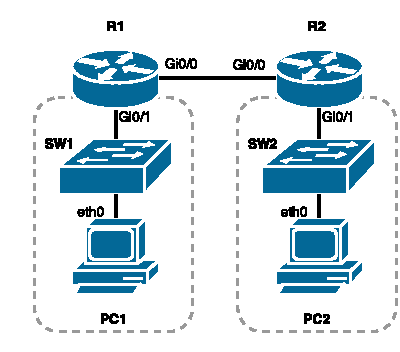
\includegraphics[width=0.6\textwidth]{figures/labtop}
            \caption{Physical lab topology.}
            \label{fig:labtop}
        \end{figure}

    \section{Lab experiments}
        \subsection{Basic IPv4 routing workflow}
            \begin{flushright}
                \textbf{[50 points]}\marginnote{\small \textbf{Note:} When done, show your
                work to the lab engineer for grading purposes.}
            \end{flushright}

            Perform the following tasks:
            \begin{itemize}
                \item Configure\footnote{\texttt{enable}, \texttt{configure
                    terminal}, \texttt{interface Gi0/0}, \texttt{ip address
                    10.0.0.1 255.255.255.0}.} \texttt{R1}'s interfaces as follows:
                    \begin{itemize}
                        \item GigabitEthernet 0/0: IPv4 address 10.0.12.1,
                            subnet mask 255.255.255.0.
                        \item GigabitEthernet 0/1: IPv4 address 10.0.1.1,
                            subnet mask 255.255.255.0.
                    \end{itemize}
                \item Configure \texttt{R2}'s interfaces as follows:
                    \begin{itemize}
                        \item GigabitEthernet 0/0: IPv4 address 10.0.12.2,
                            subnet mask 255.255.255.0.
                        \item GigabitEthernet 0/1: IPv4 address 10.0.2.1,
                            subnet mask 255.255.255.0.
                    \end{itemize}
                \item Configure\footnote{\texttt{ifconfig eth0 10.0.1.2/24}}
                    \texttt{\texttt{PC1}}'s interfaces as follows:
                    \begin{itemize}
                        \item eth0: IPv4 address 10.0.1.2,
                            subnet mask 255.255.255.0.
                    \end{itemize}
                \item Configure \texttt{\texttt{PC2}}'s interfaces as follows:
                    \begin{itemize}
                        \item eth0: IPv4 address 10.0.2.2,
                            subnet mask 255.255.255.0.
                    \end{itemize}
            \end{itemize}

            While monitoring Wireshark instances across the PCs, answer the following questions:
            \begin{enumerate}
                \item \textbf{Q:} View the routing table of
                    \texttt{R1}\footnote{\texttt{show ip
                    route}}, \texttt{R2},
                    \texttt{PC1}\footnote{\texttt{route -n}} and \texttt{PC2}. What are
                    the routing table entries?
                \item Send\footnote{\texttt{ping 10.0.2.2}} ICMP Echo messages from \texttt{PC1} to
                    \texttt{PC2}'s IP address 10.0.2.2.
                    \begin{enumerate}
                        \item \textbf{Q:} Did the \texttt{ping} command succeed?
                        \item \textbf{Q:} Did you see ARP messages? If you saw, whose
                            MAC address was attempted to be resolved?
                        \item \textbf{Q:} Did you see ICMP messages crossing the
                            network? What paths did they follow?
                        \item \textbf{Q:} If you saw ICMP messages, what are
                            the source and destination MAC address?
                        \item \textbf{Q:} View\footnote{\texttt{show mac
                            address-table}} the MAC address table of
                            switches \texttt{SW1}, do you see \texttt{PC2}'s MAC address?
                        \item \textbf{Q:} View the MAC address table of
                            switches \texttt{SW2}, do you see \texttt{PC1}'s MAC address?
                        \item \textbf{Q:} What do you conclude from this observation?
                    \end{enumerate}
                \item Send ICMP Echo messages from \texttt{PC2} to \texttt{PC1}'s IP address
                    10.0.1.2.
                    \begin{enumerate}
                        \item \textbf{Q:} Did the \texttt{ping} command succeed?
                        \item \textbf{Q:} Did you see ARP messages? If you saw, whose
                            MAC address was attempted to be resolved?
                        \item \textbf{Q:} Did you see ICMP messages crossing the
                            network? What paths did they follow?
                        \item \textbf{Q:} If you saw ICMP messages, what are
                            the source and destination MAC address?
                        \item \textbf{Q:} View the MAC address table of
                            switches \texttt{SW1}, do you see \texttt{PC2}'s MAC address?
                        \item \textbf{Q:} View the MAC address table of
                            switches \texttt{SW2}, do you see \texttt{PC1}'s MAC address?
                        \item \textbf{Q:} What do you conclude from this observation?
                    \end{enumerate}
                \item Add the default routes to \texttt{PC1} and \texttt{PC1} as follows:
                    \begin{itemize}
                        \item \texttt{PC1}: \texttt{route add -net 0.0.0.0/0 gw
                            10.0.1.1}
                        \item \texttt{PC2}: \texttt{route add -net 0.0.0.0/0 gw
                            10.0.2.1}
                    \end{itemize}
                \item \textbf{Q:} View the routing table of \texttt{PC1} and
                    \texttt{PC2}. Do
                    you see any new added routes?
                \item Send ICMP Echo messages from \texttt{PC1} to \texttt{PC2}'s IP address
                    10.0.2.2 again.
                    \begin{enumerate}
                        \item \textbf{Q:} Did the \texttt{ping} command succeed?
                        \item \textbf{Q:} Did you see ARP messages? If you saw, whose
                            MAC address was attempted to be resolved?
                        \item \textbf{Q:} Did you see ICMP messages crossing the
                            network? What paths did they follow?
                        \item \textbf{Q:} If you saw ICMP messages, what are
                            the source and destination MAC address?
                        \item \textbf{Q:} View the MAC address table of
                            switches \texttt{SW1}, do you see \texttt{PC2}'s MAC address?
                        \item \textbf{Q:} View the MAC address table of
                            switches \texttt{SW2}, do you see \texttt{PC1}'s MAC address?
                        \item \textbf{Q:} What do you conclude from this observation?
                    \end{enumerate}
                \item Send ICMP Echo messages from \texttt{PC2} to \texttt{PC1}'s IP address
                    10.0.1.2 again.
                    \begin{enumerate}
                        \item \textbf{Q:} Did the \texttt{ping} command succeed?
                        \item \textbf{Q:} Did you see ARP messages? If you saw, whose
                            MAC address was attempted to be resolved?
                        \item \textbf{Q:} Did you see ICMP messages crossing the
                            network? What paths did they follow?
                        \item \textbf{Q:} If you saw ICMP messages, what are
                            the source and destination MAC address?
                        \item \textbf{Q:} View the MAC address table of
                            switches \texttt{SW1}, do you see \texttt{PC2}'s MAC address?
                        \item \textbf{Q:} View the MAC address table of
                            switches \texttt{SW2}, do you see \texttt{PC1}'s MAC address?
                        \item \textbf{Q:} What do you conclude from this observation?
                    \end{enumerate}
                \item Using Cisco IOS commands\footnote{\texttt{enable},
                        \texttt{configure terminal}, \texttt{ip route 10.0.2.0
                    255.255.255.0 10.0.12.2}}, add the following
                    routes to R1's and R2's routing tables:
                    \begin{itemize}
                        \item R1: 
                            \begin{itemize}
                                \item Network IP: 10.0.2.0.
                                \item Netmask: 255.255.255.0
                                \item Nexthop IP address: 10.0.12.2
                            \end{itemize}
                        \item R2: 
                            \begin{itemize}
                                \item Network IP: 10.0.1.0.
                                \item Netmask: 255.255.255.0
                                \item Nexthop IP address: 10.0.12.1
                            \end{itemize}
                    \end{itemize}
                \item \textbf{Q:} View the routing table of \texttt{R1} and \texttt{R2}. Do
                    you see any new added routes?
                \item Send ICMP Echo messages from \texttt{PC1} to \texttt{PC2}'s IP address
                    10.0.2.2 again.
                    \begin{enumerate}
                        \item \textbf{Q:} Did the \texttt{ping} command succeed?
                        \item \textbf{Q:} Did you see ARP messages? If you saw, whose
                            MAC address was attempted to be resolved?
                        \item \textbf{Q:} Did you see ICMP messages crossing the
                            network? What paths did they follow?
                        \item \textbf{Q:} If you saw ICMP messages, what are
                            the source and destination MAC address?
                        \item \textbf{Q:} View the MAC address table of
                            switches \texttt{SW1}, do you see \texttt{PC2}'s MAC address?
                        \item \textbf{Q:} View the MAC address table of
                            switches \texttt{SW2}, do you see \texttt{PC1}'s MAC address?
                        \item \textbf{Q:} What do you conclude from this observation?
                    \end{enumerate}
                \item Send ICMP Echo messages from \texttt{PC2} to \texttt{PC1}'s IP address
                    10.0.1.2 again.
                    \begin{enumerate}
                        \item \textbf{Q:} Did the \texttt{ping} command succeed?
                        \item \textbf{Q:} Did you see ARP messages? If you saw, whose
                            MAC address was attempted to be resolved?
                        \item \textbf{Q:} Did you see ICMP messages crossing the
                            network? What paths did they follow?
                        \item \textbf{Q:} If you saw ICMP messages, what are
                            the source and destination MAC address?
                        \item \textbf{Q:} View the MAC address table of
                            switches \texttt{SW1}, do you see \texttt{PC2}'s MAC address?
                        \item \textbf{Q:} View the MAC address table of
                            switches \texttt{SW2}, do you see \texttt{PC1}'s MAC address?
                        \item \textbf{Q:} What do you conclude from this observation?
                    \end{enumerate}
            \end{enumerate}


            \subsection{A closer look into the IPv4
            packet}\label{sec:ipv4close}
            \begin{flushright}
                \textbf{[50 points]}\marginnote{\small \textbf{Note:} When done, show your
                work to the lab engineer for grading purposes.}
            \end{flushright}

            Using the knowledge acquired from the previous sections, send an IP
            packet from \texttt{PC1} to \texttt{PC2} (or \texttt{PC2} to
            \texttt{PC1} depending on your team's orientation) with the
            following specifications:

            \begin{itemize}
                \item Craft a MAC frame accordingly (i.e. choose the
                    approperiate source MAC address, destination MAC address,
                    type (0x0800 for IP).
                \item Inside the payload of the MAC frame, send the following
                    IP packet:
                \begin{itemize}
                    \item Version: 4,
                    \item IHL: 5 32bit words (i.e. minimal header length),
                    \item Type of Service: set to 0 (off-topic),
                    \item Total length: calculate it according to the header length
                        + payload length,
                    \item Identification: set to 0 (off-topic),
                    \item Flags: set to 0 (off-topic),
                    \item Fragment offset: set to 0 (off-topic),
                    \item Time to Live: choose the right TTL value such that it's
                        not too small to cause death of packets while being routed,
                    \item Protocol: for this lab, set it to any arbitrary number
                        (but in later labs we will set it according to the
                        next-layer's protocol),
                    \item Header cehcksum: calculate it according to the provided
                        algorithm from RFC791 as quoted in earlier sections,
                    \item Source address: set it accordingly,
                    \item Destination address: set it accordingly.
                    \item Payload: ``Hello'' (without double quotes; using
                        the ASCII table in hex, it would be \texttt{0x48, 0x65,
                        0x6C, 0x6C, 0x6F}).
                \end{itemize}
            \end{itemize}

            When done, hit \texttt{enter} if using \texttt{scapy}, or compile
            it if using \texttt{macpacketsender.c} using \texttt{gcc
            macpacketsender.c -o macpacketsender}, then execute it by
            \texttt{./macpacketsender}.

            Upon the successful execution of this task, the receiver PC should
            be able to receive the message. Make sure to share your findings to
            the lab engineer upon completion.


        \subsection{Extra questions: IPv6}\marginnote{\small
            \textbf{Note:} when done, show your answers to the lab engineer for
            feedback. If the lab time is not enough, take your time and submit it
            in a later time. Although not graded, it can strengthen your
            understanding of the subject.}

            In this section, you will be able to use your laptop to inject MAC
            packets into various VLANs.

            \subsubsection{Basic IPv6 routing workflow}
                \begin{enumerate}
                    \item Enable\footnote{\texttt{enable}, \texttt{config
                        terminal}, \texttt{ipv6 unicast-routing}} IPv6 routing on routers \texttt{R1} and
                        \texttt{R2}.
                    \item Assign IPv6 IP addresses to the router interfaces as
                        follows:
                        \begin{itemize}
                            \item \texttt{R1}'s \texttt{Gi0/0}:
                                \texttt{FD00:12::1/64}\footnote{\texttt{enable},
                                    \texttt{config terminal}, \texttt{interface
                                gi0/0}, \texttt{ipv6 address FD00:12::1/64}}
                            \item \texttt{R1}'s \texttt{Gi0/1}:
                                \texttt{FD00:1::1/64}
                            \item \texttt{R2}'s \texttt{Gi0/0}:
                                \texttt{FD00:12::2/64}
                            \item \texttt{R2}'s \texttt{Gi0/1}: 
                                \texttt{FD00:2::1/64}
                            \item \texttt{PC1}'s \texttt{eth0}: 
                                \texttt{FD00:1::2/64}\footnote{\texttt{ifconfig eth0 inet6
                                add FD00:1::2/64}}
                            \item \texttt{PC2}'s \texttt{eth0}: 
                                \texttt{FD00:2::2/64}
                        \end{itemize}
                    \item Add the routing table entries as follows:
                        \begin{itemize}
                            \item \texttt{R1}'s routing table:
                                \begin{itemize}
                                    \item IPv6 Network IP: \texttt{FD00:2::}
                                    \item IPv6 Netmask: 64 bits
                                    \item Nexthop: \texttt{FD00:12::2}
                                \end{itemize}
                            \item \texttt{R2}'s routing table: 
                                \begin{itemize}
                                    \item IPv6 Network IP: \texttt{FD00:1::}
                                    \item IPv6 Netmask: 64 bits
                                    \item Nexthop: \texttt{FD00:12::1}
                                \end{itemize}
                            \item \texttt{PC1}'s routing table (a default route
                                entry): 
                                \begin{itemize}
                                    \item IPv6 Network IP: \texttt{::}
                                    \item IPv6 Netmask: 0 bits
                                    \item Nexthop: \texttt{FD00:1::1}
                                \end{itemize}
                            \item \texttt{PC2}'s routing table (a default route
                                entry): 
                                \begin{itemize}
                                    \item IPv6 Network IP: \texttt{::}
                                    \item IPv6 Netmask: 0 bits
                                    \item Nexthop: \texttt{FD00:2::1}
                                \end{itemize}
                        \end{itemize}
                    \item Verify the configurations:
                        \begin{itemize}
                            \item \texttt{R1}'s routing
                                table\footnote{\texttt{enable}, \texttt{show ipv6
                                route}}.
                            \item \texttt{R2}'s routing table.
                            \item \texttt{PC1}'s routing
                                table\footnote{\texttt{enable}, \texttt{route -A
                                inet6 -n}}.
                            \item \texttt{PC2}'s routing table.
                        \end{itemize}
                    \item Send an ICMP Echo from \texttt{PC1} to \texttt{PC2}'s
                        IPv6 address\footnote{\texttt{ping6 FD00:2::2}}
                \end{enumerate}

                You should then able to successfully receive IPv6 ICMP Echo and
                Echo-Reply messages across \texttt{PC1} and \texttt{PC2}.

            \subsubsection{A closer look into IPv6 packets}
                This is an easy task as the IPv6 header contains a lot less
                fields, and particularly no Checksum field.

                Repeat the task from Section \ref{sec:ipv4close} except for
                applying IPv6's packet format as depicted in Figure
                \ref{fig:ipv6}



\end{document}
